\section{measurements}
\subsection{Techniques used for the evaluation}
All calculations in this section are done with scripts written in 
the \textit{python} programming language~\cite{python}, relaying in several 
packages:
\begin{itemize}
    \item
        \textit{matplotlib}~\cite{Hunter2007} for plotting,
    \item
        \textit{scipy}~\cite{scipy} for fitting, and 
    \item
        \textit{uncertainties}~\cite{uc} for error propagation.
\end{itemize}
The latter applies gaussian error propagation for correlated and uncorrelated variables. 
We will thus not explicitly write down the formulas for the error propagation 
for each quantity calculated but instead state the numerical result, only. 
We will, however make a quick remark on the use of covariance matrices in 
error propagation: Contrary to measured data, which in our case is usually 
expected to be uncorrelated, all fitted data yields variables that in general correlate. 
The propagation is then done as follows:
Let's assume we have random
variables $x_0,...,x_N$ which are correlated through the $N\times N$ Matrix $cov(x_i,x_j)$.
For a scalar function $f(x_0,...,x_N) \rightarrow \mathbb{R}$, the variance is estimated (linearly) by:
\begin{equation}
Var[f] = \sigma^2 = \sum_{i,j} \frac{\partial f}{\partial x_i} \frac{\partial f}{\partial x_j} cov(x_i,x_j) \,.
\end{equation} 
If instead, $\mathbf{f}$ is a vector field in $m$ dimensions, namely 
$\mathbf{f}(x_0,...,x_N) \rightarrow \mathbb{R}^m$, then the components of $\mathbf{f}$ 
are further correlated. We can write down the relation between the covariance matrices $V$ and $U$ of 
$\mathbf{x}$ and $\mathbf{f}$, respectively, in matrix relations:
\begin{equation}
    U = A V A^T
\end{equation}
where $A$ is the matrix defined by 
\begin{equation}
    A_{ij} = \left[ \frac{\partial f_i}{\partial x_j}\right]_{\mathbf{x} = \mathbf{\mu}}
\end{equation}
with expectation value $E[\mathbf{x}] = \mathbf{\mu}$.~\cite{cowan1998statistical}
In order to facilitate notation, the covariance matrices will in general be notated without 
specifying the units. If not specified explicitly, the units will correspond to those of the
variables: If $x_i, x_j$ have the units $[x_i], [x_j]$, respectively, 
then the entry of the covariance matrix has the unit $[x_i] * [x_j]$. 


\subsection{Calibration and preparation}
As it was already described we performed the calibration in order to maximize the amplitude of the
signal, which was the case for \\
\begin{align*}
     \mathrm{VCA} &= 1355 \qquad \text{(Amplitude of the RLC circuit)}\\
     \mathrm{VCO} &= 1422 \qquad\text{(Frequency of the RLC circuit)}\\ 
     \mathrm{Offset} &= 1680 \qquad\text{(Offset for shifting the signal)}\\
     \mathrm{FB-R} &= 50 k \qquad \text{(Feedback resistor)}
\end{align*}
For the given constraints of the experimental setup see figure~\ref{fig:setup1}.
\begin{figure}[htpb]
    \centering
    \includegraphics[width=0.8\linewidth]{figures/setup1}
    \caption{Experimental constraints, which we measured before the experimental procedure. The squid
    is connected to the controlling unit, whose output we observe on the oscilloscope. The oscillscope
    is additionally connected to the computer in order for us to analyze the output of the squid even further.}
    \label{fig:setup1}
\end{figure}
\\\\
We have measured the radius of the coil to be 
\begin{equation}
r = \frac{d}{2} = (2.0 \pm 0.25) \mathrm{mm}
\end{equation}
Using the approximation from equation \eqref{eq:aprox1} we can calculate the
magnetic field with 
\begin{align}
B_z     &= \frac{\mu_0\cdot I \cdot r^2}{2z^3} = \frac{\mu_0\cdot U \cdot r^2}{2Rz^3}\\ 
p       &= \pi r^2 U / R 
\end{align}
Where the we estimate the distance between SQUID and sample with
\begin{equation}
z = \left[ 3.0 \pm 0.5 \right]\mathrm{mm}
\end{equation}
\begin{table}[htb]
\caption{Calculated magnetic fields of the induction loop}
\begin{tabular}{ l| p{2cm}|p{2cm}|p{2cm}|p{2cm}|p{2cm}}
 \rowcolor{tabcolor}& R1 & R2 & R3 & R4 & R5 \\ 
Resistance / $\Omega$ & 51.47  $\pm 0.05$ & 100.8  $\pm 0.1$& 300.8 $\pm 0.3$& 510.6 $\pm 0.3$ & 1000 $\pm 1$\\  
Voltage U/V           & 2.63 $\pm 0.01$ & 2.67 $\pm 0.01$& 2.70 $\pm 0.01$& 2.70 $\pm 0.01$& 2.71 $\pm 0.01$\\
Magnetic field $B_{\mathrm{il}}$ / nT &$4.6\pm1.5$&$2.5\pm0.8$&$0.8\pm0.3$&$0.5\pm0.2$&$0.3\pm0.1$ \\ 
Dipole moment $p_{\mathrm{il}}$ / C$\cdot$nm&$617. \pm 150$&$332 \pm 80$&$112 \pm 30$&$66 \pm 20$&$34 \pm 8$\\
\end{tabular}
\end{table}

\subsection{Measurements with the SQUID}

In order to get a reasonable estimation for the amplitude, we use a least
squares fit with the functional
\begin{equation}
A \dot \sin (\omega t - \phi ) + c
\end{equation}
with the parameters $A$, $\omega$, $\phi$ and $c$. This parameterspace can be
reduced by setting the offset of the data to zero. This is possible by a 
smoothing method: Before further analysis, we smooth the data with a
Savitzky-golay filter\footnote{The Savitzky-golay filter is broadly used
in order to smmooth data without changing the characteristic features of the 
signal. The method is a combination of convolution and polynomial least
squares fitting.} in order to estimate the parameters for 
subtracting the estimation for $c$, so are left with
\begin{equation}
A \dot \sin (\omega t - \phi ) 
\end{equation}
The other paramters will be given as
first guess for another least squares fit, now with the real data. This
described method worked very well for us, since the guess of the filtered data
provides the following least squares fit with a good deal of information and
results in a promosing fit (see figure\ref{fig:setup1}). 

\begin{figure}[H]
    \centering
    \includegraphics[width=1\linewidth]{analysis/figures/fit4_1}
    \caption{Selected measurement (R1) in order to visualize the least squares
    fitting. For the other measurements please see the appendix.}
    \label{fig:4_1_plot}
\end{figure}

For calculating the magnetic field, we can use \cite{ver} that
the feedback resistor $s_i [V/\phi_0]$ is connected by the effective area $A_{\mathrm{eff}}$
with the magnetic field, such that
\begin{equation}
B_z = F \frac{\Delta V}{s_i} 
\end{equation}
where we used the Flux coefficient $F = 9.3$nT$/\phi_0$ (given by the manufactorer) 
instead of the effective area, connected by $F = A_{\mathrm{eff}}^{-1}$.
\begin{table}[htb]
\caption{Calculated magnetic fields of the induction loop}
\begin{tabular}{ l| p{2.3cm}|p{2.3cm}|p{2.3cm}|p{2.3cm}|p{2.3cm}}
 \rowcolor{tabcolor}& R1 & R2 & R3 & R4 & R5 \\ 
Resistance / $\Omega$ & 50  $\pm 1$ & 100  $\pm 1$& 300  $\pm 1$& 500 $\pm 1$ & 1000 $\pm 1$\\  
Amlitude / mV &$273.7 \pm 0.7$&$142.1 \pm 0.6$&$48.2 \pm 0.5$&$27.9 \pm 0.5$&$15.4 \pm 0.7$\\
Magnetic field $B_{\mathrm{sq}}$ / nT &$5.09 \pm 0.12$&$2.64 \pm 0.06$&$0.896 \pm 0.022$&$0.519 \pm 0.015$&$0.286 \pm 0.014$\\  
Dipole mom. $p_{\mathrm{sq}}$/ C$\cdot$nm &$690 \pm 140$ & $360 \pm 70$ &$121 \pm 24$ & $70 \pm 14$ & $39 \pm 8$ \\
\end{tabular}
\end{table}

\begin{table}[htb]
\caption{Comparison of the two methods. ``il'' denotes to induction loop method, while ``sq'' denotes to SQUID method.}
\begin{tabular}{ l| p{2.3cm}|p{2.3cm}|p{2.3cm}|p{2.3cm}|p{2.3cm}}
 \rowcolor{tabcolor}& R1 & R2 & R3 & R4 & R5 \\ 
$B_{\mathrm{il}}$ / nT &$4.7\pm1.5$&$2.5\pm0.8$&$0.8\pm0.3$&$0.5\pm0.2$&$0.3\pm0.1$ \\ 
$p_{\mathrm{il}}$ / C$\cdot$nm&$617 \pm 150$&$332 \pm 80$&$112 \pm 30$&$66 \pm 20$&$34 \pm 8$\\ \hline
$B_{\mathrm{sq}}$ / nT &$5.09 \pm 0.12$&$2.64 \pm 0.06$&$0.896 \pm 0.022$&$0.519 \pm 0.015$&$0.286 \pm 0.014$\\  
$p_{\mathrm{sq}}$ / C$\cdot$nm &$690 \pm 140$ & $360 \pm 70$ &$121 \pm 24$ & $70 \pm 14$ & $39 \pm 8$ \\ 
\end{tabular}
\end{table}

\begin{table}[htb]
\caption{Measuring the magnetic field of different materials (We changed the unit within three orders of magnitude).}
\begin{tabular}{ l| p{2.3cm}|p{2.3cm}|p{2.3cm}|p{2.3cm}|p{2.3cm}}
 \rowcolor{tabcolor}& Gold & Iron & Gold  & Stick & Magnet splint \\ 
Amplitude / V &$0.046 \pm 0.005$&$0.054 \pm 0.005$&$0.051 \pm 0.005$&$3.72 \pm 0.05$&$6.94 \pm 0.04$\\
$B_{\mathrm{sq}}$ / $\mu$T  &$0.86 \pm 0.09$ &$1.00 \pm 0.10$ &$0.95 \pm 0.10$ &$69.2 \pm 1.8$ &$129.2 \pm 3.0$ \\ 
$p_{\mathrm{sq}}$ / C$\cdot\mu$m  &$0.116 \pm 0.026$&$0.136 \pm 0.030$&$0.128 \pm 0.029$&$9.3 \pm 1.9$&$17 \pm 4$\\
\end{tabular}
\end{table}








